\begin{frame}\begin{center}
    \LARGE\textbf{Human Capital}
\end{center}\end{frame}
%-------------------------------------------------------------------------------
%-------------------------------------------------------------------------------
\begin{frame}
Human capital is defined as:
\vspace{\baselineskip}

\begin{quote}
The knowledge, skills, competencies and attributes embodied in individuals that facilitate
the creation of personal, social and economic well-being.
\end{quote}\vspace{-0.5pt} \hspace{6cm} - OECD (2001)
\end{frame}
%-------------------------------------------------------------------------------
%-------------------------------------------------------------------------------
\begin{frame}\begin{center}
\LARGE\textit{Basics}
\end{center}\end{frame}
%-------------------------------------------------------------------------------
%-------------------------------------------------------------------------------
\begin{frame}
We study the basic relationship between basic measures of human capital and wages at age thirty-five.
\end{frame}
%-------------------------------------------------------------------------------
%-------------------------------------------------------------------------------
\begin{frame}
\begin{itemize}
\item The \textbf{Armed Forces Vocational Aptitude Test Battery} (ASVAB) is a multiple-aptitude battery that measures developed abilities and helps predict future academic and occupational success in the military.
\begin{multicols}{2}
\begin{itemize}\setlength\itemsep{1em}
\item Arithmetic reasoning
\item Paragraph comprehen.
\item Word knowledge
\item Math knowledge
\item Coding speed
\end{itemize}
\end{multicols}
\end{itemize}

\end{frame}
%-------------------------------------------------------------------------------
%-------------------------------------------------------------------------------
\begin{frame}
\begin{itemize}
\item The \textbf{ Armed Forces Qualifications Test (AFQT)} is considered a general measure of trainability based on the ASVAB. It has been used extensively as a measure of cognitive skills in the literature.
\end{itemize}
\end{frame}

%-------------------------------------------------------------------------------
%-------------------------------------------------------------------------------
\begin{frame}\begin{figure}[htp]\centering
\caption{AFQT Score}
\scalebox{0.35}{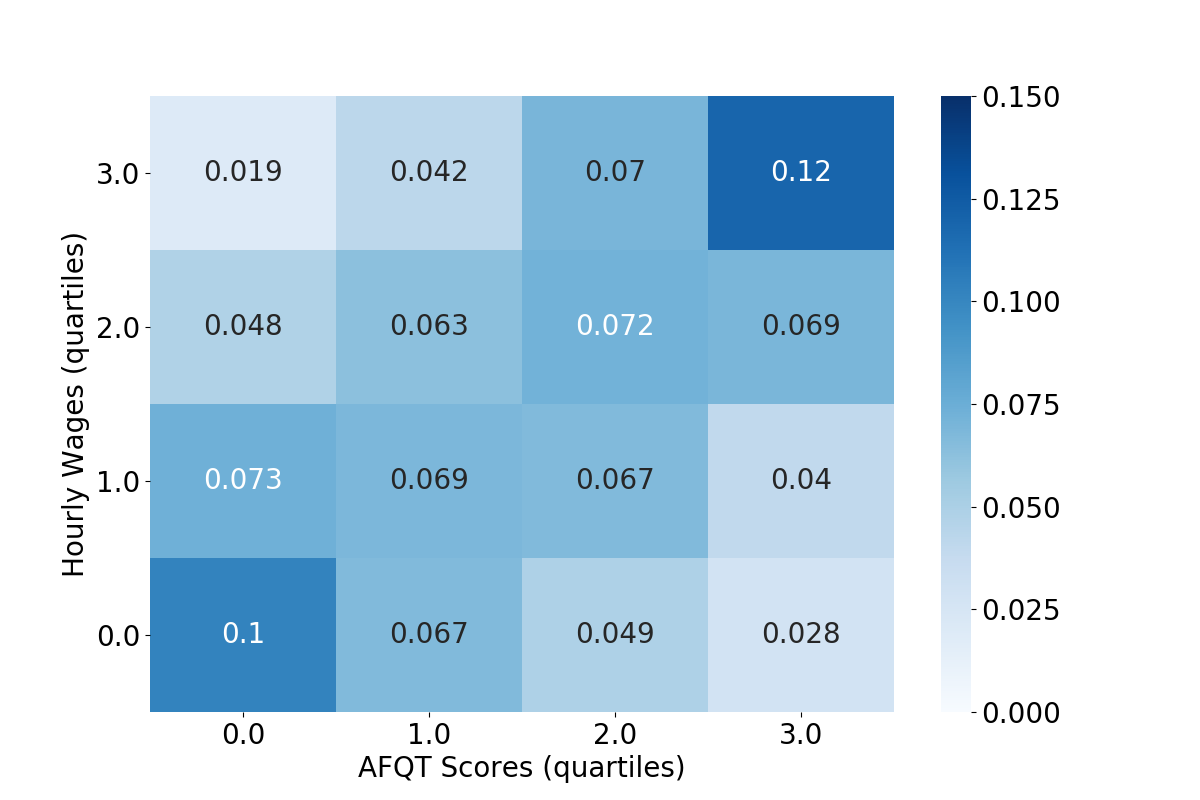
\includegraphics{fig-human-capital-basic-afqt}}
\end{figure}\end{frame}
%-------------------------------------------------------------------------------
%-------------------------------------------------------------------------------
\begin{frame}
\begin{itemize}
\item The \textbf{Rotter scale} \citep{Rotter.1966} measures the degree of control individuals feel they
possess over their life and has been used in previous studies analyzing
the role of noncognitive skills on labor outcomes.
\end{itemize}
\end{frame}
%-------------------------------------------------------------------------------
%-------------------------------------------------------------------------------
\begin{frame}\begin{figure}[htp]\centering
\caption{Rotter Score}
\scalebox{0.35}{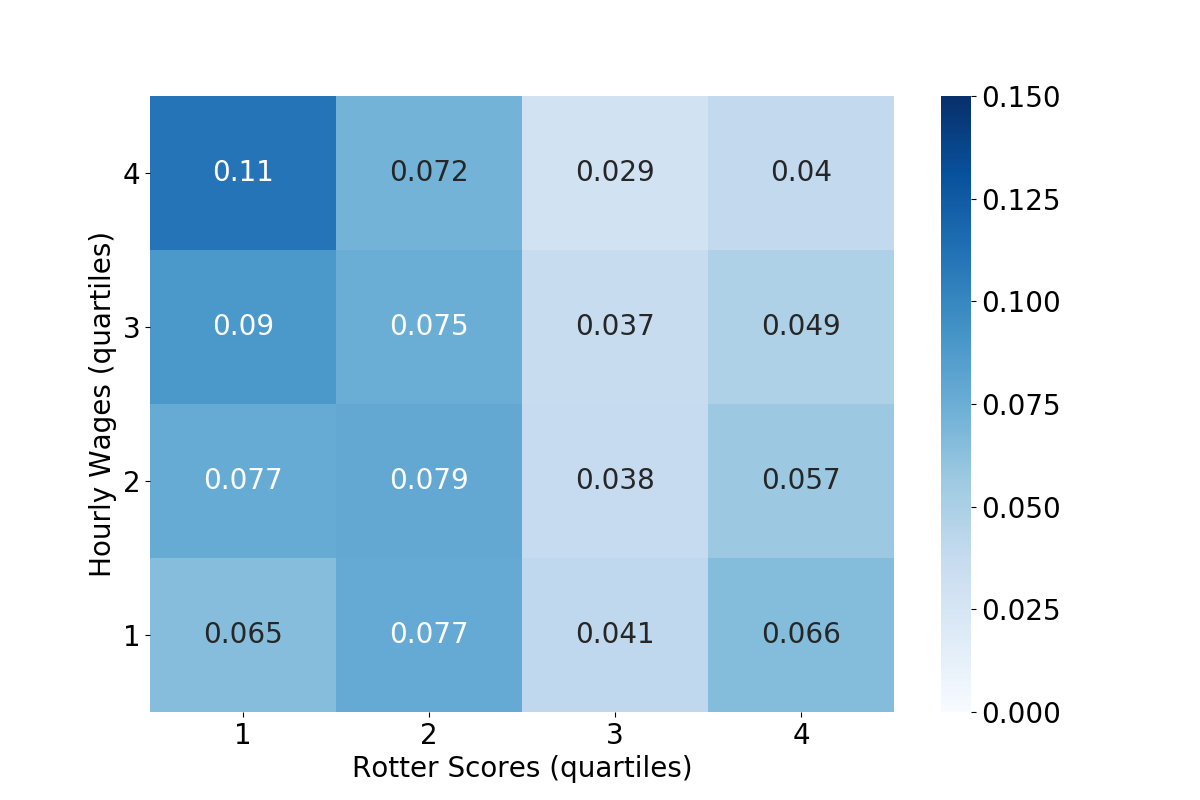
\includegraphics{fig-human-capital-basic-rotter}}
\end{figure}\end{frame}
%-------------------------------------------------------------------------------
%-------------------------------------------------------------------------------
\begin{frame}
\begin{itemize}
\item The \textbf{Rosenberg scale} \citep{Rosenberg.1965} measures perceptions of self-worth.
\end{itemize}
\end{frame}
%-------------------------------------------------------------------------------
%-------------------------------------------------------------------------------
\begin{frame}\begin{figure}[htp]\centering
\caption{Rosenberg Score}
\scalebox{0.35}{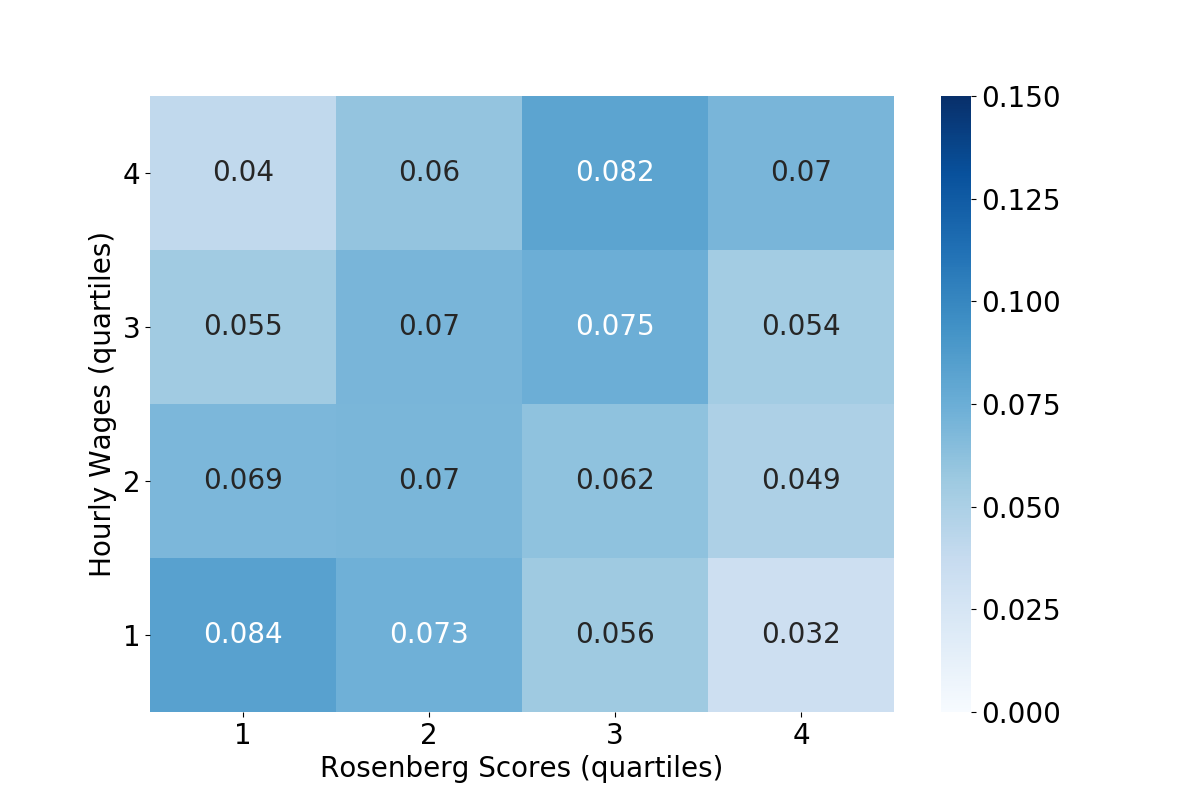
\includegraphics{fig-human-capital-basic-rosenberg}}
\end{figure}\end{frame}
%-------------------------------------------------------------------------------
%-------------------------------------------------------------------------------
\begin{frame}\begin{center}
\LARGE\textit{Differences by income quartile}
\end{center}\end{frame}
%-------------------------------------------------------------------------------
%-------------------------------------------------------------------------------
\begin{frame}\begin{figure}[htp]\centering
\caption{AFQT Score}
\scalebox{0.35}{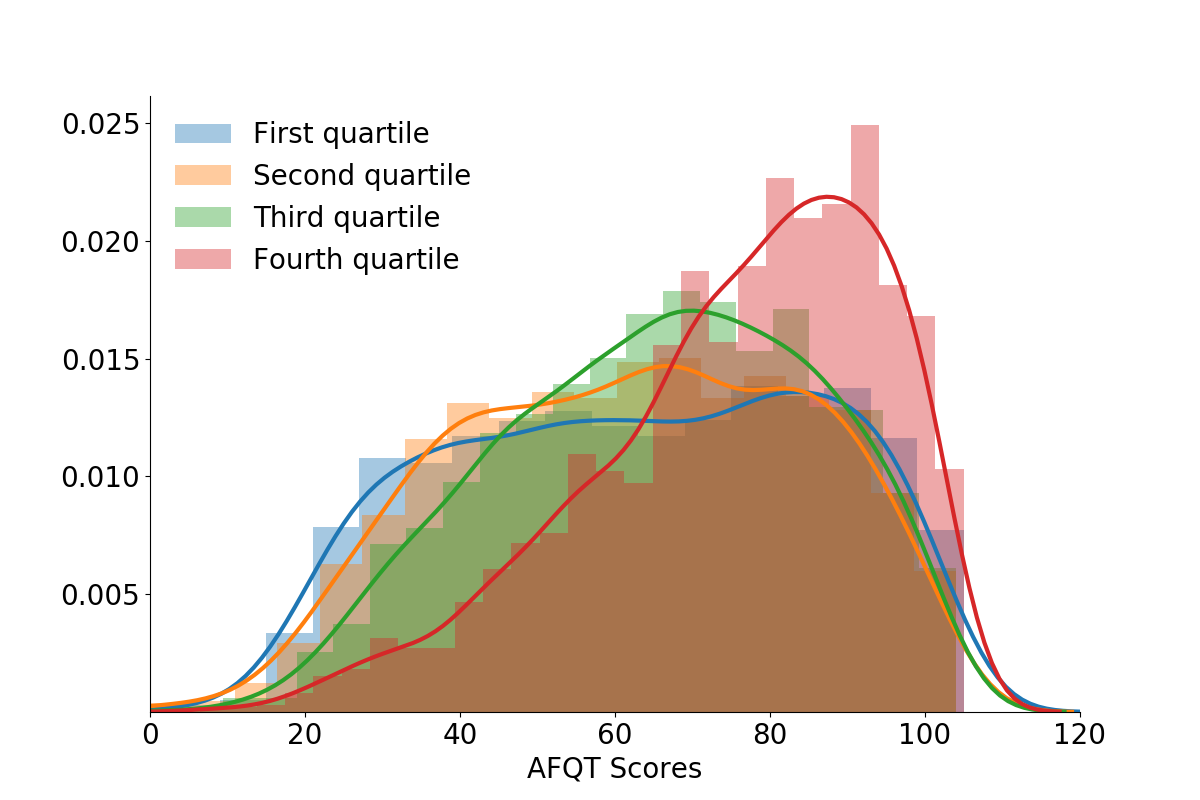
\includegraphics{fig-human-capital-income-quartile-afqt}}
\end{figure}\end{frame}
%-------------------------------------------------------------------------------
%-------------------------------------------------------------------------------
\begin{frame}\begin{figure}[htp]\centering
\caption{Rotter Score}
\scalebox{0.35}{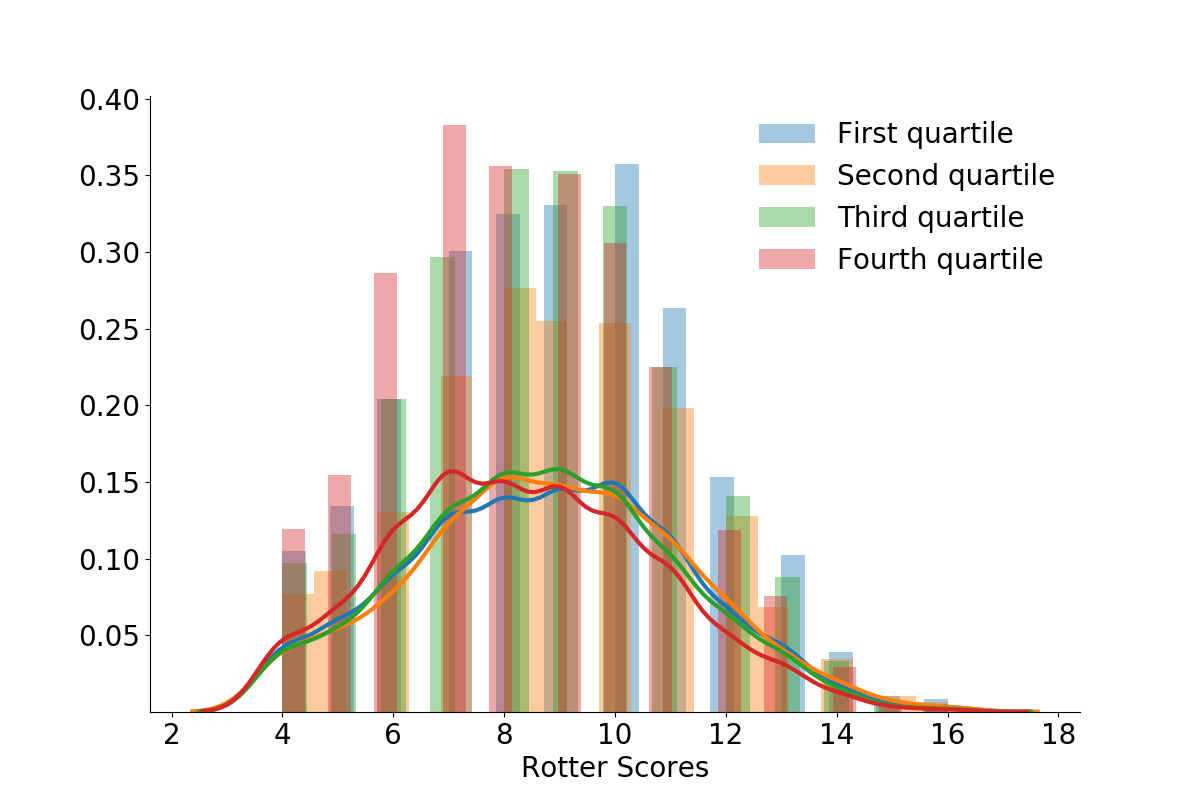
\includegraphics{fig-human-capital-income-quartile-rotter}}
\end{figure}\end{frame}
%-------------------------------------------------------------------------------
%-------------------------------------------------------------------------------
\begin{frame}\begin{figure}[htp]\centering
\caption{Rosenberg Score}
\scalebox{0.35}{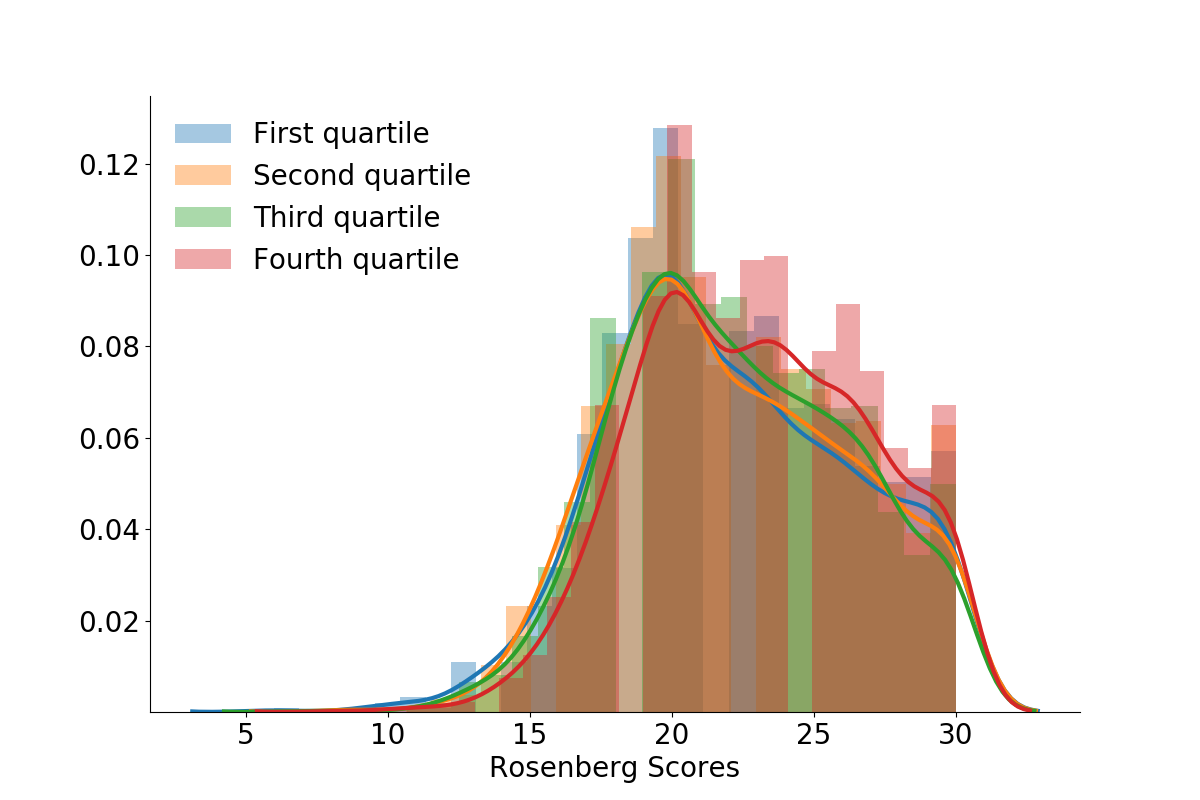
\includegraphics{fig-human-capital-income-quartile-rosenberg}}
\end{figure}\end{frame}
%-------------------------------------------------------------------------------
%-------------------------------------------------------------------------------
\begin{frame}\textbf{Research Questions}\vspace{0.3cm}
\begin{itemize}\setlength\itemsep{1em}
\item What is driving the observed differences in these test scores?
\end{itemize}
\end{frame}
%-------------------------------------------------------------------------------
%-------------------------------------------------------------------------------
\begin{frame}\begin{center}
\LARGE\textit{Intergenerational Transmission}
\end{center}\end{frame}
%-------------------------------------------------------------------------------
%-------------------------------------------------------------------------------
\begin{frame}\begin{figure}[htp]\centering
\caption{Father's education}
\scalebox{0.35}{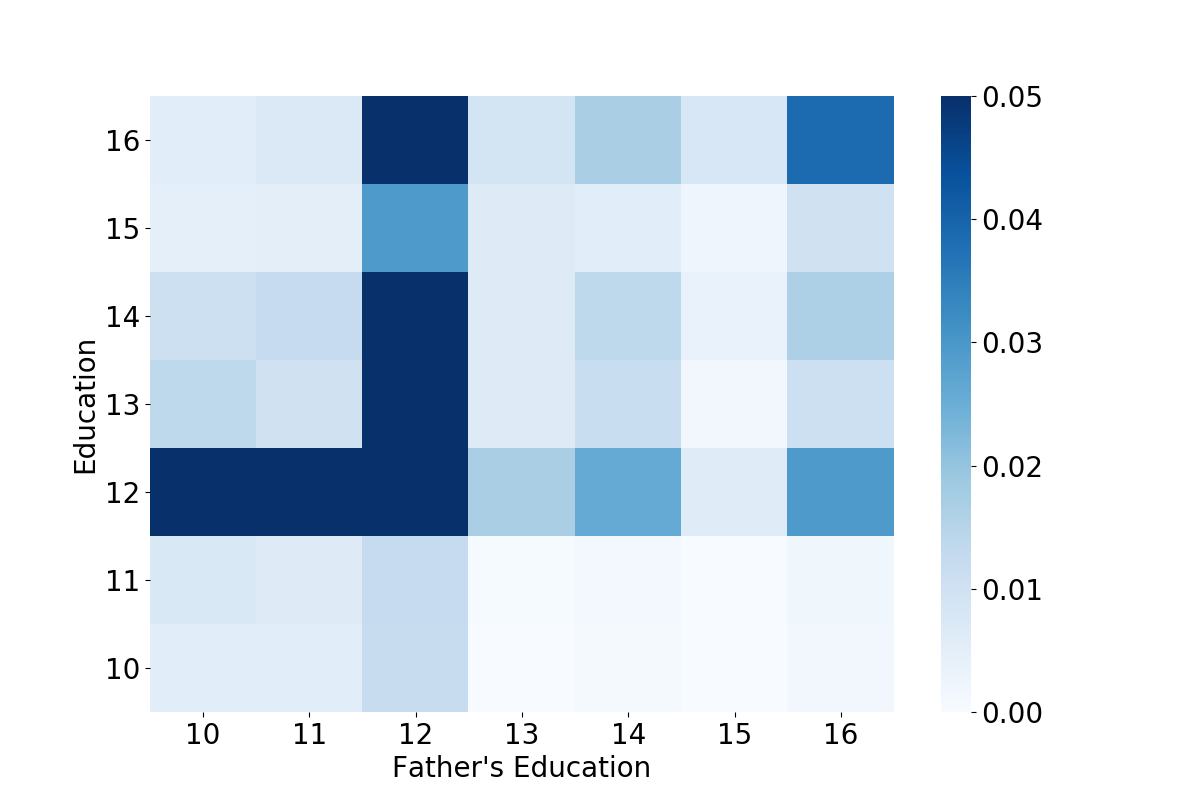
\includegraphics{fig-human-capital-intergenerational-father}}
\end{figure}\end{frame}
%-------------------------------------------------------------------------------
%-------------------------------------------------------------------------------
\begin{frame}\begin{figure}[htp]\centering
\caption{Mother's education}
\scalebox{0.35}{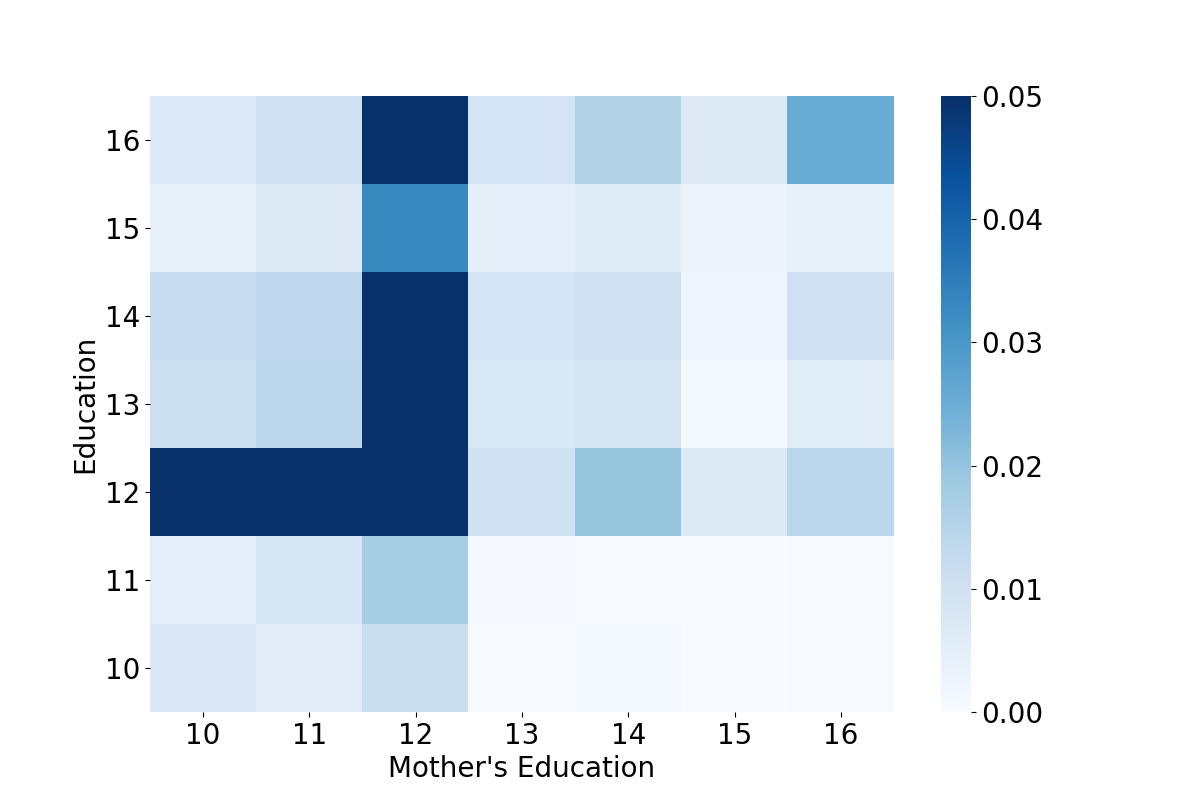
\includegraphics{fig-human-capital-intergenerational-mother}}
\end{figure}\end{frame}
%-------------------------------------------------------------------------------
%-------------------------------------------------------------------------------
\begin{frame}\textbf{Research Questions}\vspace{0.3cm}
\begin{itemize}\setlength\itemsep{1em}
\item What are the mechanisms driving the intergenerational correlation of human capital?
\item How does the relationship evolve over time?
\item Are there any suitable policy responses to consider?
\end{itemize}
\end{frame}
%-------------------------------------------------------------------------------
%-------------------------------------------------------------------------------
